\section{Procesos}
\subsection{Introduccion}

Un proceso es una abstracción de un programa en ejecución, que básicamente convierte una CPU en varias CPU virtuales, proporcionando de esta manera la capacidad de operar (pseudo)concurrentemente, incluso cuando hay una sola CPU disponible.

Un proceso no es más que una instancia de un programa en ejecución, incluyendo los valores actuales del contador de programa, los registros y las variables. En concepto, cada proceso tiene su propia CPU virtual; en la realidad, la CPU real conmuta de un proceso a otro. Varios procesos pueden compartir un solo procesador mediante el uso de un algoritmo de planificación para determinar cuándo se debe detener el trabajo en un proceso para dar servicio a otro.

Hay cuatro eventos principales que provocan la creación de procesos:
\begin{itemize}
\item El arranque del sistema
\item La ejecución de una llamada al sistema para creación de procesos.
\item Una petición de usuario para crear un proceso.
\item El inicio de un trabajo por lotes.
\end{itemize}

Algunos procesos corren en primer plano, es decir, interactúan con los usuarios, mientras que otros procesos, que no están asociados con usuarios específicos sino con una función específica, corren en segundo plano. Un ejemplo sería un proceso que acepte peticiones entrantes para las páginas web hospedadas en ese equipo; estos procesos se conocen como \textbf{daemons}.

En UNIX sólo hay una llamada al sistema para crear un proceso: \textbf{fork}. Esta llamada crea un clon exacto del proceso que hizo la llamada. Después del fork, los dos procesos (padre e hijo) tienen la misma imagen de memoria, las mismas variables de entorno y los mismos archivos abiertos. Por lo general, el proceso hijo ejecuta después a \textbf{execve} o una llamada al sistema similar para cambiar su imagen de memoria y ejecutar un nuevo programa. La razón de este proceso de dos pasos es para permitir al hijo manipular sus descriptores de archivo después de fork, pero antes de execve, para poder lograr la redirección de la entrada, salida y error estándar.

\subsection{Estados de un proceso}

Un proceso se puede encontrar en uno de tres estados:

\begin{itemize}
\item En ejecución (está usando la CPU en ese instante)
\item Listo (ejecutable. Se detuvo temporalmente para dejar que se ejecute otro proceso.)
\item Bloqueado (no puede ejecutarse hasta que ocurra cierto evento externo)
\end{itemize}

~\\
\begin{figure}[h]
	\begin{center}
	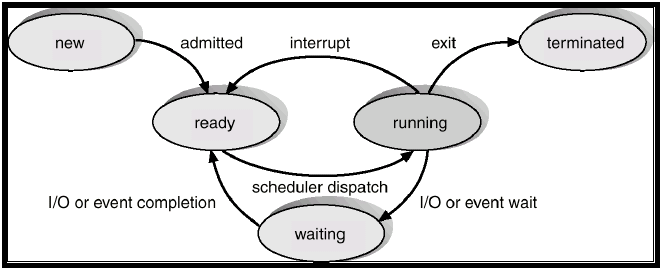
\includegraphics[width=0.8\textwidth]{imagenes/processstates.png}
	\caption{Estados de un proceso}
	\end{center}
\end{figure}
~\\

\subsection{Implementación de los procesos}

Para implementar el modelo de procesos, el SO mantiene una tabla llamada tabla de procesos, con una entrada por cada proceso (llamada Process Control Block (PCB)). Esta entrada contiene información importante acerca del estado de cada proceso, como el Program Counter, el Stack Pointer, asignación de memoria, estado de sus archivos abiertos, información para el scheduler, registros de la CPU, etc.

Cuando ocurre una interrupción, el PC, el PSW, y uno o más registros se meten en la pila mediante el hardware de interrupción. Después, la CPU salta a la dirección especificada en el vector de interrupción. Esto es todo lo que hace el hardware, en adelante es todo responsabilidad del software.

Todas las interrupciones comienzan por guardar los registros, a menudo en la entrada de la tabla de procesos para el proceso actual. Después, se quita la información que la interrupción metió en la pila y el stack pointer se establece para que apunte a una pila temporal utilizada por el manejador de procesos.

Cuando se terminan de guardar los registros, se llama a un procedimiento para realizar el resto del trabajo para este tipo de interrupción específica. Cuando termina su trabajo y tal vez algún otro proceso está listo, el scheduler es llamado para ver qué proceso se debe ejecutar a continuación. Después de eso, el control pasa de vuelta al código en lenguaje ensamblador para cargar los registros y el mapa de memoria para el proceso que entonces es el actual.

Un resumen de los pasos que ejecuta el sistema operativo cuando ocurre una interrupción es el siguiente:

\begin{enumerate}[1]
\item[1)] El hardware mete el PC, PSW, registros, etc. a la pila.
\item[2)] El hardware carga el nuevo PC del vector de interrupciones.
\item[3)] Procedimiento en lenguaje ensamblador guarda los registros.
\item[4)] Procedimiento en lenguaje ensamblador establece la nueva pila.
\item[5)] El servicio de interrupciones de C se ejecuta.
\item[6)] El scheduler decide qué proceso se va a ejecutar a continuación.
\item[7)] Procedimiento en C regresa al código en ensamblador.
\item[8)] Procedimiento en lenguaje ensamblador inicia el nuevo proceso actual.
\end{enumerate}

A continuación un ejemplo de una interrupción en el contexto de una syscall:

~\\
\begin{figure}[h]
	\begin{center}
	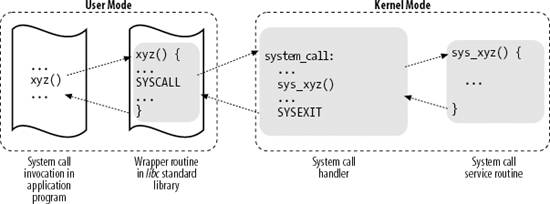
\includegraphics[width=0.8\textwidth]{imagenes/syscall.png}
	\caption{syscall}
	\end{center}
\end{figure}
~\\

\subsection{Threads}

Los threads son una especie de "mini roceso" o "proceso ligero" dentro de un proceso clásico. Los threads posibilitan el concepto de procesos secuenciales que realizan llamadas al sistema con bloqueo y de todas formas logran paralelismo.

Una manera de ver a un proceso es como si fuera una forma de agrupar recursos relacionados, como archivos abiertos, procesos hijos, etc., además de su espacio de direcciones. El otro concepto que tiene un proceso es el de hilo de ejecución, el cual tiene un contador de programa, registros con sus variables actuales y una pila. Aunque un hilo se deba ejecutar en cierto proceso, el hilo y su proceso son conceptos distintos y pueden tratarse por separado.

Lo que agregan los hilos al modelo de procesos es permitir que se lleven a cabo varias ejecuciones en el mismo entorno del proceso, que son en gram parte independientes, por lo tanto, los hilos dentro de un proceso comparten el mismo espacio de direcciones. No hay protección entre los hilos debido a que (1) es imposible y (2) no debe ser necesario. A diferencia de tener procesos diferentes, que pueden ser de distintos usuarios y hostiles entre sí, un proceso siempre es propiedad de un solo usuario, quien se supone ha creado varios hilos para que cooperen. Además de compartir un espacio de direcciones, todos los threads pueden compartir el mismo conjunto de archivos abiertos, procesos hijos, señales, etc. Al igual que un proceso tradicional, un thread puede estar en uno de varios estados: ene ejecución, bloqueado, listo o terminado.

Hay 2 formas principales de implementar una librería de threads: en espacio de usuario o en el kernel, aunque también es posible una implementación híbrida.

\subsubsection{Implementación de threads en espacio de usuario}

En este caso la librería de threads reside completamente en espacio de usuario, y el kernel no sabe nada de ellos. En lo que al kernel concierne, está administrando procesos ordinarios con un solo thread.

En este caso, cada proceso tiene su propia tabla de threads. Algunas ventajas son que cuando un thread se bloquea y se debe conmutar con otro, el procedimiento es mucho más rápido que hacer el trap al kernel. Otra ventaja es que cada proceso puede tener su propio algoritmo de planificación personalizado.

A pesar de su buen rendimiento, los threads a nivel de usuario tienen algunos problemas importantes. El primero de todos es la manera en que se implementan las llamadas al sistema de bloqueo. Si, por ejemplo, un thread lee del teclado antes de que se haya oprimido una sola tecla, es inaceptable permitir que el thread se bloquée, ya que esto también bloqueará a todos los threads del proceso. Si un thread produce un fallo de página, el kernel naturalmente bloquea a todo el proceso, llevando al mismo problema que en el caso anterior.

Otro problema es que si un thread comienza a ejecutarse, ningún otro thread en ese proceso se ejecutará a menos que el primero renuncie de manera voluntaria a la CPU, ya que dentro de un proceso no hay interrupciones.

\subsubsection{Implementación de threads en el kernel}

En este caso, en vez de tener una tabla de threads por proceso, el kernel tiene una tabla de threads que lleva la cuenta de todos los threads del sistema. Además, el kernel mantiene la tabla de procesos tradicional. Cuando un proceso desea crear un nuevo thread, realiza una llamada al kernel. Los threads del kernel no requieren de nuevas llamadas al sistema no bloqueantes, y si se produce un fallo de página, el kernel puede comprobar con facilidad si el proceso tiene otros threads que puedan ejecutarse y los ejecuta. Su principal desventaja es que el costo de una llamada al sistema es considerable. Sin embargo, hay algunos problemas que no resuelven, como qué hacer luego de un fork, o qué hilo debe hacerse cargo de una señal enviada al proceso.

\subsubsection{Implementaciones híbridas}

Una manera de combinar los métodos anteriores es utilizar threads de nivel kernel y después multiplexar los threads de nivel usuario con alguno o todos los threads de nivel kernel. El programador puede determinar cuántos hilos de kernel va a utilizar y cuántos threads de nivel usuario va a multiplexar en cada uno.


\subsection{Sincronización entre procesos}

Los bugs